\begin{center}
    \vspace*{1.5cm}
    {\fontsize{20}{20}\textbf{Andra sektioners visor}}\\
    \vspace{0.7cm}
    {\fontsize{12}{12}\textit{Om [insert sektion] själv får välja}}  
\end{center}
\addtocwithheader{Andra sektioners visor}  % Add entry to TOC and set header\noBackground
\newpage
\resetBackground

\begin{comment}
\subsubsection*{Kul info om andra sektioner}

Här ska vi skriva kul info om andra sektioner och att de har maskotar mm.

Vill vi skriva om TLTH också och att de också har färg och djur?

Uppmana till att andra visor är bra. cos(x) bra för endimen.

\newpage
\end{comment}
\noBackground
\subsection*{Andra sektioner}

Varje sektion har sin egen färg och varsitt skyddshelgon, vilka listas nedan.

\renewcommand{\arraystretch}{1.3}
\setlength{\tabcolsep}{10pt}

\begin{center}
\begin{tabular}{lll}
\textbf{Sektion} & \textbf{Färg} & \textbf{Skyddshelgon} \\

F-sektionen & Orange & Hilbert Älg \\
E-sektionen & Vit & Hacke Hackspett \\
M-sektionen & Röd & Joe Cool \\
V-sektionen & Blå & Vincent Ralén \\
A-sektionen & Lila & Skalman \\
K-sektionen & Gul & Miraculix \\
D-sektionen & Rosa & Rosa Pantern \\
Dokt-sektionen & Silver & Dr And \\
ING-sektionen & Mörkblå & Rune Andréasson \\
W-sektionen & Turkos & Wera Haj \\
I-sektionen & Vinröd & I:s björn \\
\end{tabular}
\end{center}

Det är alltid kul att sjunga E-visor, men man får inte glömma av att man kan lära sig många andra roliga låtar från andra sektioner när man lärt känna dem. 
F har t.ex. en kul om ko-sex (läs: \(\cos(x)\)) som man alltid bör komma ihåg under Endim-tentorna.

\vissteduatt{Visste du att Teknologkåren är den kår som har haft kårstatus \\allra längst i Lund?}

\newpage
\resetBackground
% Detta fungerar inte riktigt än. Något blir knas med krusidull-E:et på varannan sida
\backgroundsetup{
  scale=0.40,
  opacity=0.15,
  angle=0,
  color=black,
  vshift=-230,
  hshift=160,
  contents={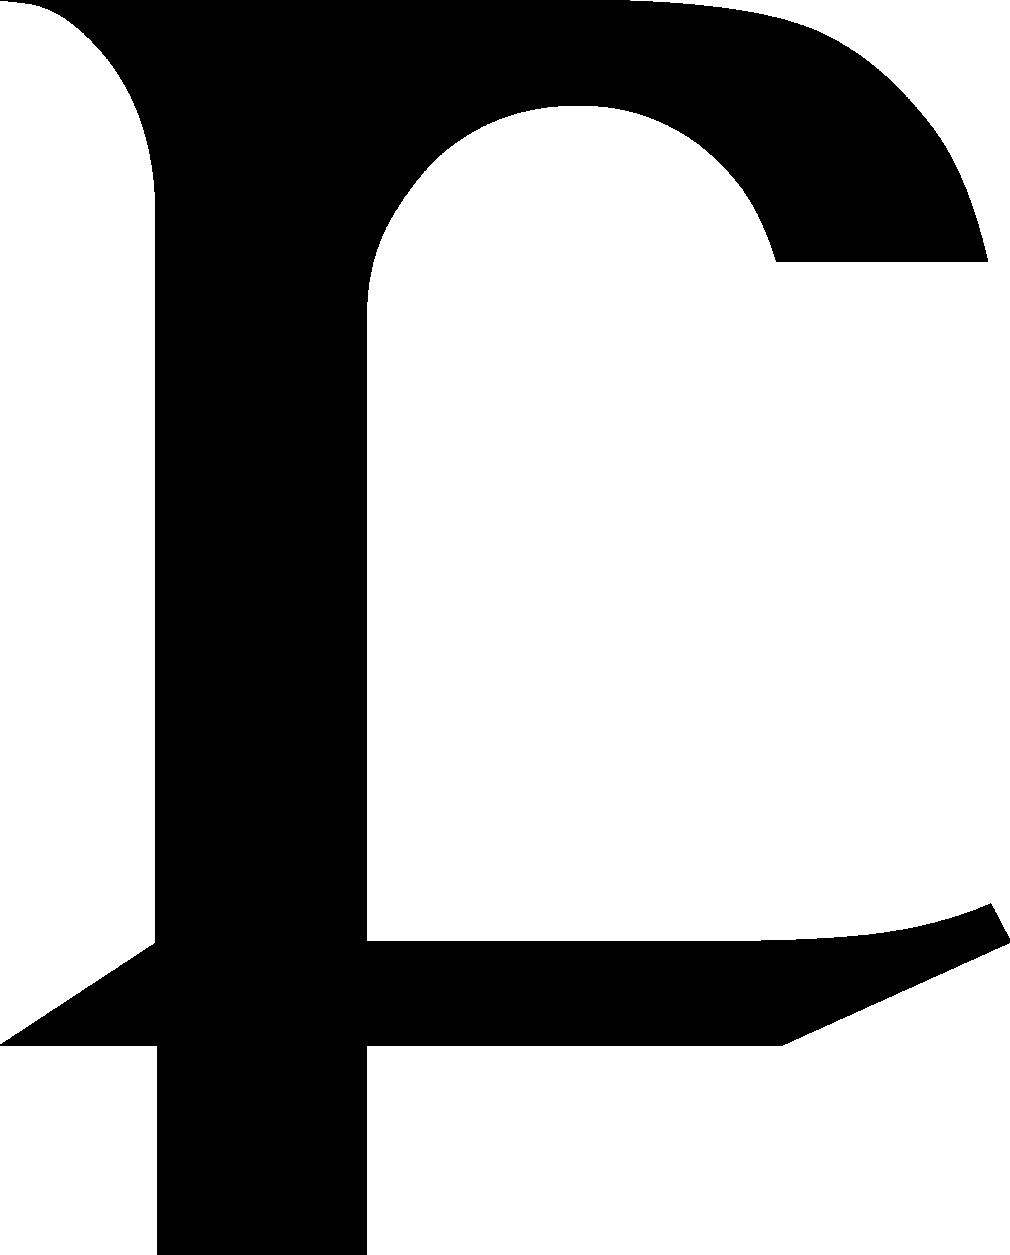
\includegraphics[width=\paperwidth]{./bilder/sektions_bilder/F.png}}
}

\subsection*{Hyllningsvisa till teknisk fysik} 
\index[alfa]{Hyllningsvisa till teknisk fysik}
\index[anfa]{Teknisk Fysik är mössbeklädda töntar}
\songinfo{Mel: Sit on my face}

\begin{parse lines}[\noindent]{#1\\}
    Teknisk Fysik är mössbeklädda töntar,
    fula flickor och en samling mammas pojkar.
    Liknar mest en televerksbil, som gått för många mil,
    en teknisk fossil.

    Teknisk Fysik är lättare än att fjärta,
    döda älgar värmer nu mitt kalla hjärta.
    Ta hit dynamit, spräng teknik, vårt gebit.
    Dessa tofsprydda avskum som ger oss kolik!
    Dessa tofsprydda avskum som ger oss kolik!
    Dessa tofsprydda avskum som ger oss kolik!
    Dessa tekniska lik!
    Barambam!
    
\end{parse lines}

\subsection*{Vi går på F-sek} 
\index[alfa]{Vi går på F-sek}
\index[anfa]{kosex}

\begin{parse lines}[\noindent]{#1\\} 

    Vi går på F-sek, F-sek vi går på F-sek
    Derivera sin($x$) så får du cos($x$)
    cos($x$) cos($x$) vi vill ha cos($x$)
    Vill vi? Neeej!
    Vi går på F-sek, F-sek vi går på F-sek
    Derivera sin($x$) så får du cos($x$)
    cos($x$) cos($x$) vi vill ha cos($x$)
    Vill vi? Neeej, vi vill ha ÄLGSEX!
\end{parse lines}

\vissteduatt{Visste du att de första E:arna nollades av F:are?}

\newpage
\resetBackground
% \noBackground

\subsection*{Supa tills vi stupar} 
\index[alfa]{Supa tills vi stupar}
\index[anfa]{Vi öla på Malmö}
\songinfo{Mel: The wild rover}

\begin{parse lines}[\noindent]{#1\\}
    Vi öla på Malmö, till sång och till skrik
Då kom det en grabb, han gick juridik
Han kom fram till vårt bord, kalla oss fulla svin
men det skiter vi i för vi går på Maskin

Vi blir kvar och röjer
Kommer aldrig gå hem
Vi ska supa tills vi stupar
För vi går på M

Vi öla i parken, då kom det en man
Han hade fått sparken, var sliten som fan
Han sa "Läs inte data. Ni slösar bort ti’n"
Men det skiter vi i för vi går på Maskin

Vi blir kvar...

Vi öla på Sparta, som så ofta har hänt
Då kom det en östtysk utbytesstudent
Han sa "Tjänare grabbar, vill ni ha lite morfin?"
Nej det skiter vi i, TROTS vi går på Maskin

Vi blir kvar...
\end{parse lines}
\newpage


\backgroundsetup{
  scale=0.40,
  opacity=0.15,
  angle=0,
  color=black,
  vshift=-230,
  hshift=160,
  contents={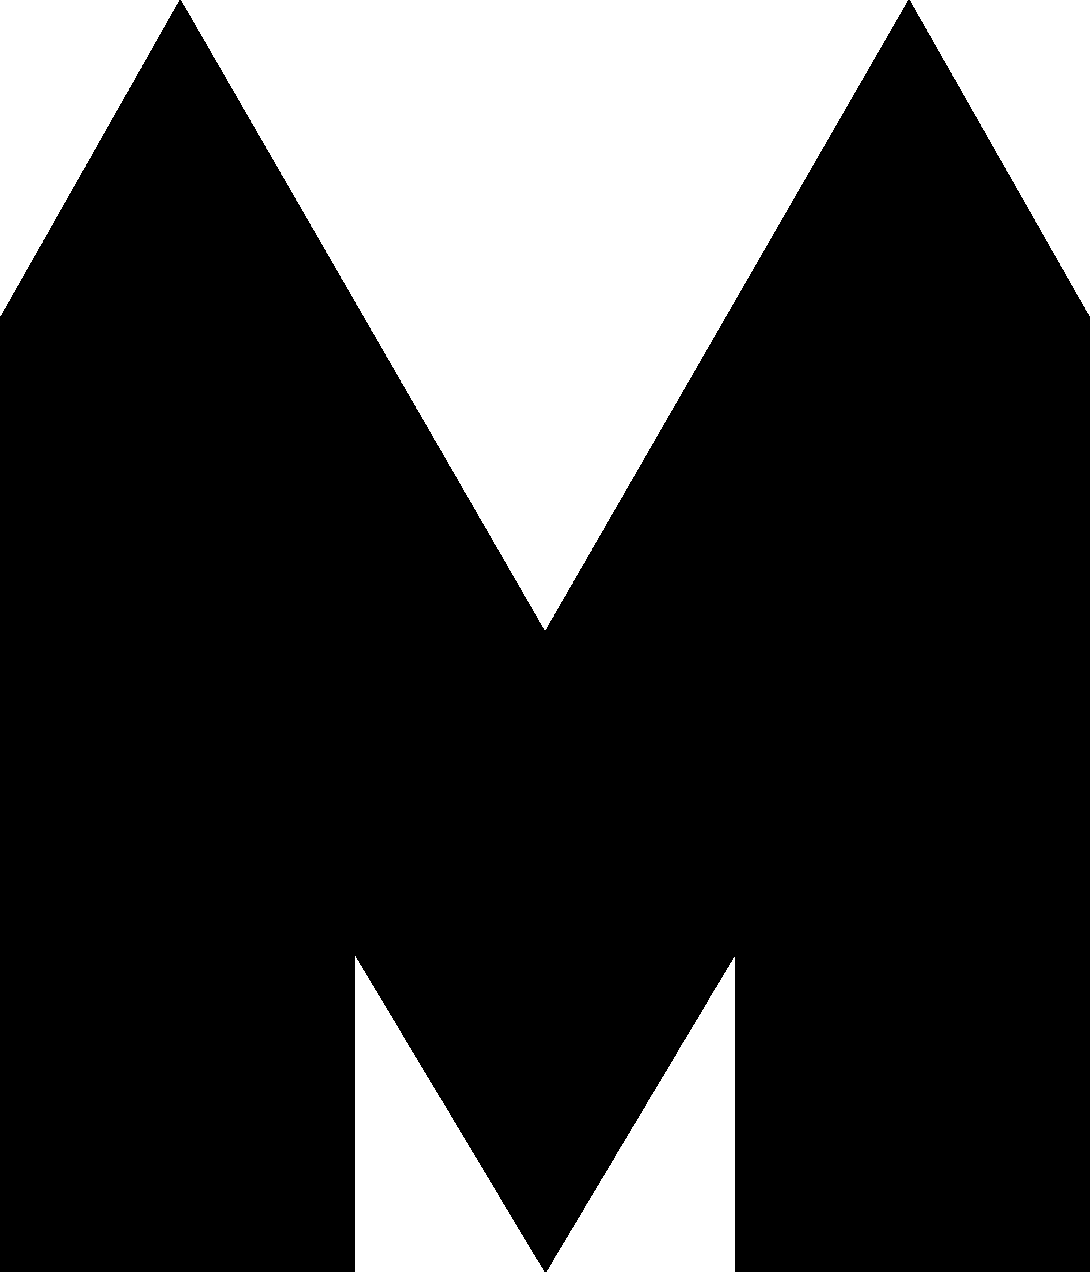
\includegraphics[width=\paperwidth]{./bilder/sektions_bilder/M.png}}
}


\begin{parse lines}[\noindent]{#1\\}
Vi vakna på sjukan, hur fan kom vi dit?
Men där kom nå’n på här finns ju läkarsprit
Men doktorn sa "Stopp! Det där är till medicin!"
Men det skiter vi i för vi går på Maskin

Vi blir kvar...

\end{parse lines}


\subsection*{Vår färg är röd} 
\index[alfa]{Vår färg är röd}
\index[anfa]{Vår färg är röd}
\songinfo{Mel: When the saints go marching in}

\begin{parse lines}[\noindent]{#1\\}
    Vår färg är röd, vår färg är fin,
    för det är vi som går Maskin
    Och vi har kommit för att dricka alkohol,
    för det är vi som går Maskin

\end{parse lines}

\vissteduatt{Visste du att M-sektionen fick en gammal frys av E-sektionen i \\
50-års present, som E-sektionen ville bli av med?}


\newpage
\resetBackground
% \resetBackground % ------------------------------------------------------- reset background
\backgroundsetup{
  scale=0.50,
  opacity=0.15,
  angle=0,
  color=black,
  vshift=-180,
  hshift=110,
%   vshift=-230,
%   hshift=160,
  contents={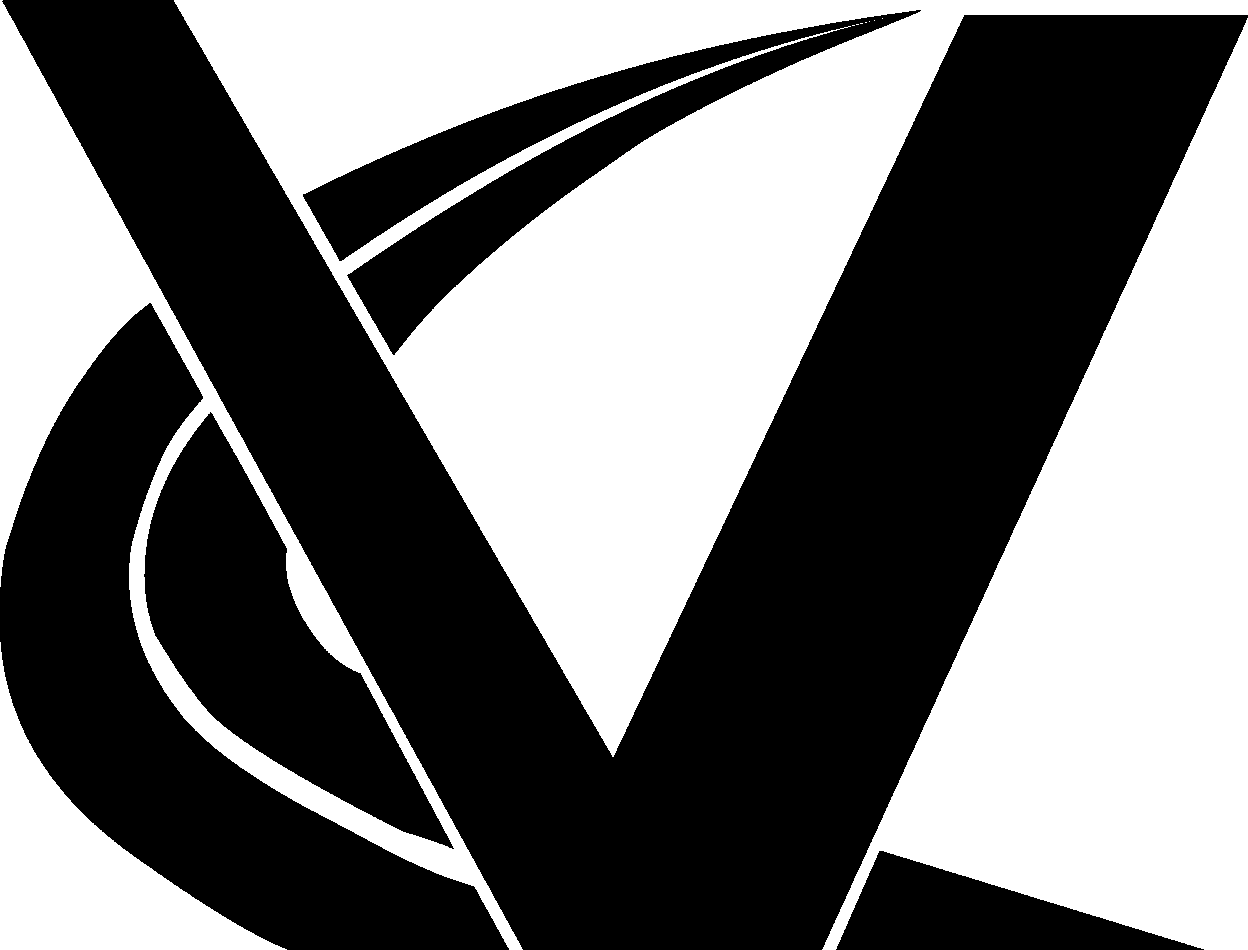
\includegraphics[width=\paperwidth]{./bilder/sektions_bilder/V.png}}
}

\subsection*{V-ingenjören} 
\index[alfa]{V-ingenjören}
\index[anfa]{V-ingenjören}
\songinfo{Mel: Sovjets nationalsång (nästan)}

\begin{parse lines}[\noindent]{#1\\}
    Gudarnas gunstling, så stark, klok och sann.
    Från falsk blygsamhet vi ska er förskona, 
    vi vet vad vi vill och vi vet vad vi kan. 

    Vi bygger bro mellan fjärran stränder. 
    Vi drar en väg mellan alla länder.
    En väg mellan folken, en strålande syn.
    Vi skapar kraft, tämjer syndafloden. 
    Vår jord bebyggt så man kan bebo den, 
    Från klingfasta berget mot strålande blånande? skyn.

    Skåla kamrater, skål för varandra. 
    Skål ingenjörer av sten och av stål. 
    Vi breddar vartefter den vägen vi vandra. 
    Vårt mål är en skål, så skål för vårt mål. 

    Vi bygger bro…
\end{parse lines}

\subsection*{För vi är de blå} 
\index[alfa]{För vi är de blå}
\index[anfa]{För vi är de blå}
\songinfo{Mel: Das rote Pferd}

\begin{parse lines}[\noindent]{#1\\}
    ||: FÖR… VI… ÄR… de blå, och vi är inte små
    Nej vi störst och bäst på hela LTH
    Shalalala lala
    Shalalala lala
    Shalalala la la la la lalalalala :||
\end{parse lines}
\vissteduatt{Visste du att F:s sektionsvisa skrevs av V-sektionen till \\
en Sångarstrid?}
\newpage
\resetBackground

\subsection*{Av med ouverallen} 
\index[alfa]{Av med ouverallen}
\index[anfa]{Av med ouverallen}
\songinfo{Mel: Ingen har sett fantomen}

\begin{parse lines}[\noindent]{#1\\}
    Ingen har sett ett I-Phøs utan pengar,
    kuddar av sedlar, kashmir i sina sängar.
    Han drar pappas kort på Lunds nation
    när han vaskar champagnen i hon.
    
    Ingen har sett ett W-Phøs gå i otakt,
    svin mot sina nollor, gråter över valjakt.
    Dreadlocks, tofu \& minkar ut ur bur,
    blir adopterade av Moder Natur.
    
    Av med ouverallen, det är inte minusgrader,
    du är över tio, jobbar inte på ett lager.
    Gör som A-Phøs skaffa en kavaj, 
    det ser bättre ut på varje partaj!
    
    Ingen har sett ett E-Phøs hela och rena,
    bajs i håret och lera över bena.
    Hygien gör väl ingenting, 
    det finns ändå inga damer omkring.
    
    Ingen har sett ett D-Phøs mitt på dagen,
    är framför Warcraft, ständigt helt upptagen.
    IRL är ett skrämmande begrepp,
    men kvinnorna på Sims gör mig pepp.
    
    Av med ouverallen...
\end{parse lines}

\newpage

\backgroundsetup{
  scale=0.50,
  opacity=0.15,
  angle=0,
  color=black,
  vshift=-180,
  hshift=110,
%   vshift=-230,
%   hshift=160,
  contents={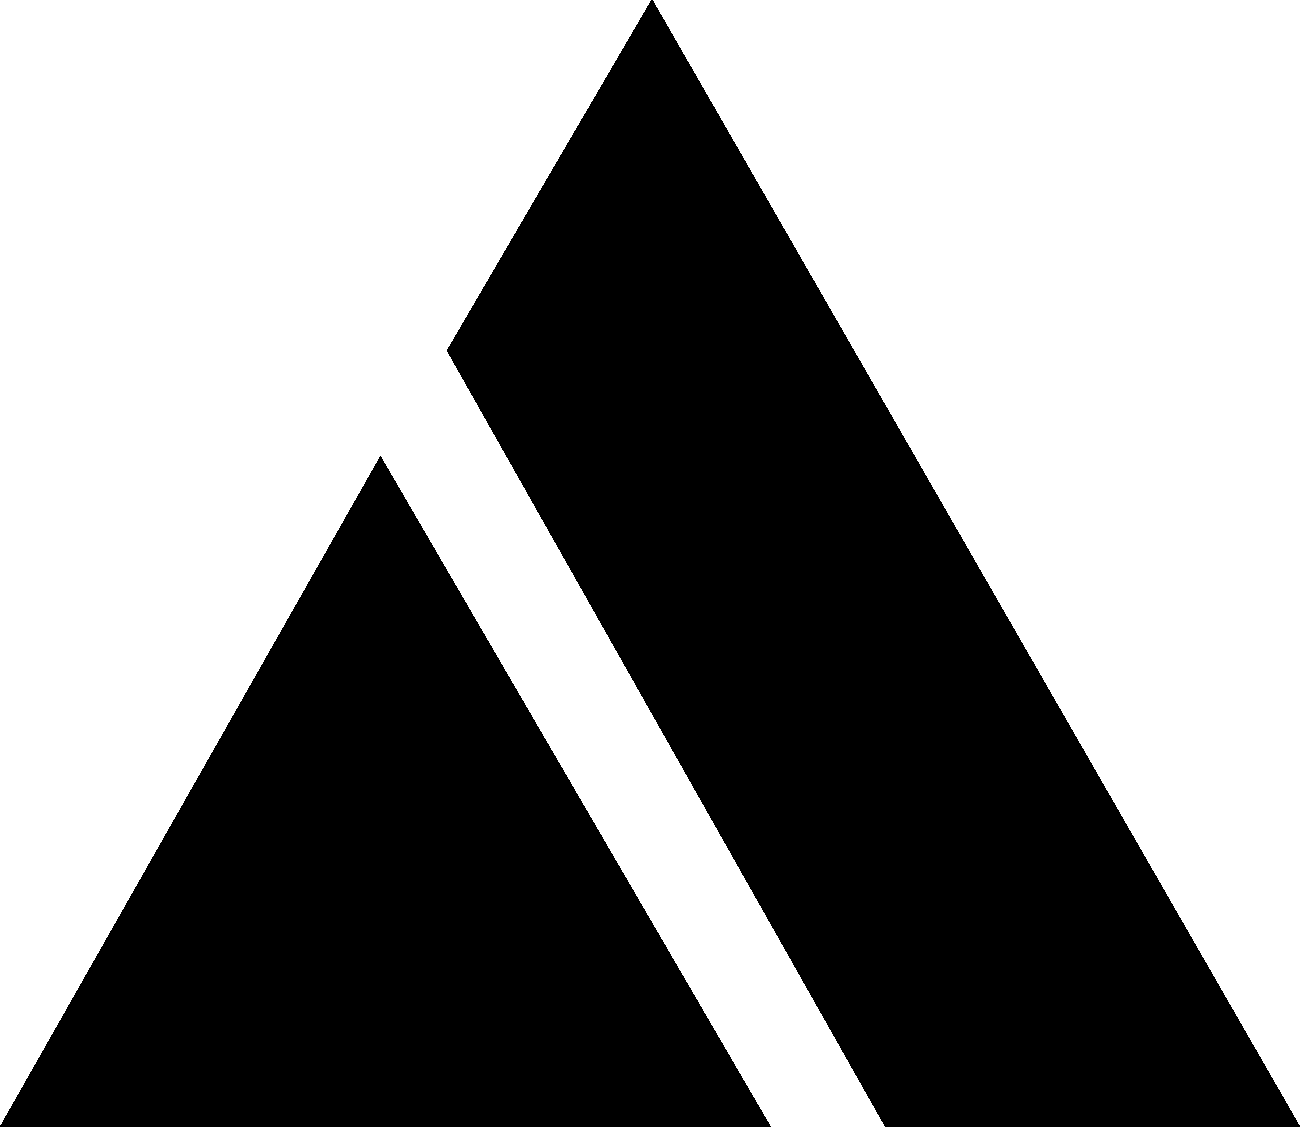
\includegraphics[width=\paperwidth]{./bilder/sektions_bilder/A.png}}
}

\begin{parse lines}[\noindent]{#1\\}
    Ingen har sett ett K-Phøs stå och skratta,
    skriker och gormar, hur fan ska nollan fatta?
    Kärleksbrygd - enda chans för en druid,
    till att bryta LTH:s nollefrid.

    Ingen har sett ett ING-Phøs
    …
    …
    …

    Av med ouverallen...

    Ingen vill se ett M-Phøs sjukjournaler
    AIDS, streptokocker och täppta tarmkanaler.
    Försöker penetrera så fort han bara kan,
    en parodi på en tvättäkta man.

    En mamma och en pappa fick ett klychigt foster, 
    villa, Volvo, vovve, till gudmor fick han moster.
    IQ under medel, kär i en blond tös,
    denna pojke är numera V-Phøs.

    Av med ouverallen...

    Ingen har sett ett F-Phøs innan teknis, 
    högstadiet var en enda social miss.
    Alkohol, bröst och en och annan dans,
    Skåne är eran sista chans.
\end{parse lines}

\newpage
\resetBackground

\begin{parse lines}[\noindent]{#1\\}
    Aldrig har ett A-Phøs skämtat om sig själva,
    har inte tid, är i skolan minst till elva.
    Klipper och klistrar får ändå CSN,
    och linjalerna får ersätta män.

    Vi vill ju faktiskt också ha en sparkdräkt,
    önskar gemenskap i eran LTH-sekt.
    Ber om förlåtelse genom alkohol, 
    och utbringar för er en stor skål!

\end{parse lines}

%\vissteduatt{fint om A-sek}

%\newpage

\subsection*{A-visan} 
\index[alfa]{A-visan}
\index[anfa]{A-sektionen den skiner såsom solen}
\songinfo{Mel: Rule, Britannia!}

\begin{parse lines}[\noindent]{#1\\}
    A-sektionen
    den skiner såsom solen
    A-sek är grym på fest
    ja A-sek är bäst

\end{parse lines}

\subsection*{A-sekt} 
\index[alfa]{A-sekt}
\index[anfa]{Vår färg är lila}
\songinfo{Mel: When the Saints Go Marching In}

\begin{parse lines}[\noindent]{#1\\}
    Vår färg är lila.
    Vi är en sekt.
    För vi går ID å Arkitekt.
    Och vi har kommit för att rita raka streck,
    för vi går ID å Arkitekt.
\end{parse lines}

\vissteduatt{Visste du att programmet i industriell design sponsras av IKEA?}

\newpage

\backgroundsetup{
  scale=0.40,
  opacity=0.15,
  angle=0,
  color=black,
  vshift=-230,
  hshift=160,
  contents={
\includegraphics[width=\paperwidth]{./bilder/sektions_bilder/K.png}}
}

\subsection*{Kemisternas kampvisa} 
\index[alfa]{Kemisternas kampvisa}
\index[anfa]{Vi är kemister}
\songinfo{Mel: Eslövs nationalvisa}

\begin{parse lines}[\noindent]{#1\\} 
Vi är kemister och vi älskar maskinister
Vi är kemister och vi pussar arkitekt
Vi är kemister och vi kramar väg och vatten
Vi är kemister och vi är allra bäst!

Å.. spela, spela data!
Å.. heja, heja F!
Å.. koppla in Elektro!
Å.. men K är allra bäst!

\end{parse lines}


\subsection*{K K} 
\index[alfa]{K K}
\index[anfa]{K K}
\songinfo{Mel: Drunken Sailor}

\begin{parse lines}[\noindent]{#1\\}  
Vilka har den starka røsten
Vilka har de størsta brøsten
Vilka ger er alltid trøsten
När ert lag førlorar

K, K, vi alla gillar
K, K, har faktiskt killar
K, K, som gärna pillar
Med sin labbutrustning

\end{parse lines}

\vissteduatt{\colorbox{yellow}{fint om k-sek}}

\newpage
\resetBackground

\subsection*{Rosa på bal} 
\index[alfa]{Rosa på bal}
\index[anfa]{Rosa på bal}
\songinfo{Evert Taube}

\begin{parse lines}[\noindent]{#1\\}
    Tänk att jag dansar med Andersson,
lilla jag, lilla jag,
med Fritiof Andersson
Tänk att bli uppbjuden av en så'n
populär person

Tänk, vilket underbart liv, det ni för
Säg mig, hur känns det att vara charmör,
sjöman och cowboy, musiker, artist
Det kan väl aldrig bli trist?

Nej, aldrig trist, fröken Rosa,
har man som er kavaljer
Vart jag än ställer min kosa,
aldrig förglömmer jag er

Ni är en sångmö från Helikons berg
Åh, fröken Rosa, er linje, er färg,
skuldran, profilen med lockarnas krans,
ögonens varma glans

Tänk, inspirera herr Andersson,
lilla jag, inspirera Fritiof Andersson
Får jag kanhända min egen sång,
lilla jag, nå'n gång?

\end{parse lines}

\vissteduatt{Visste du att "Rosa" alltid sjunges som färgen "råsa" och att \\rimmen justeras därefter?}
\newpage

\backgroundsetup{
  scale=0.40,
  opacity=0.15,
  angle=0,
  color=black,
  vshift=-230,
  hshift=160,
  contents={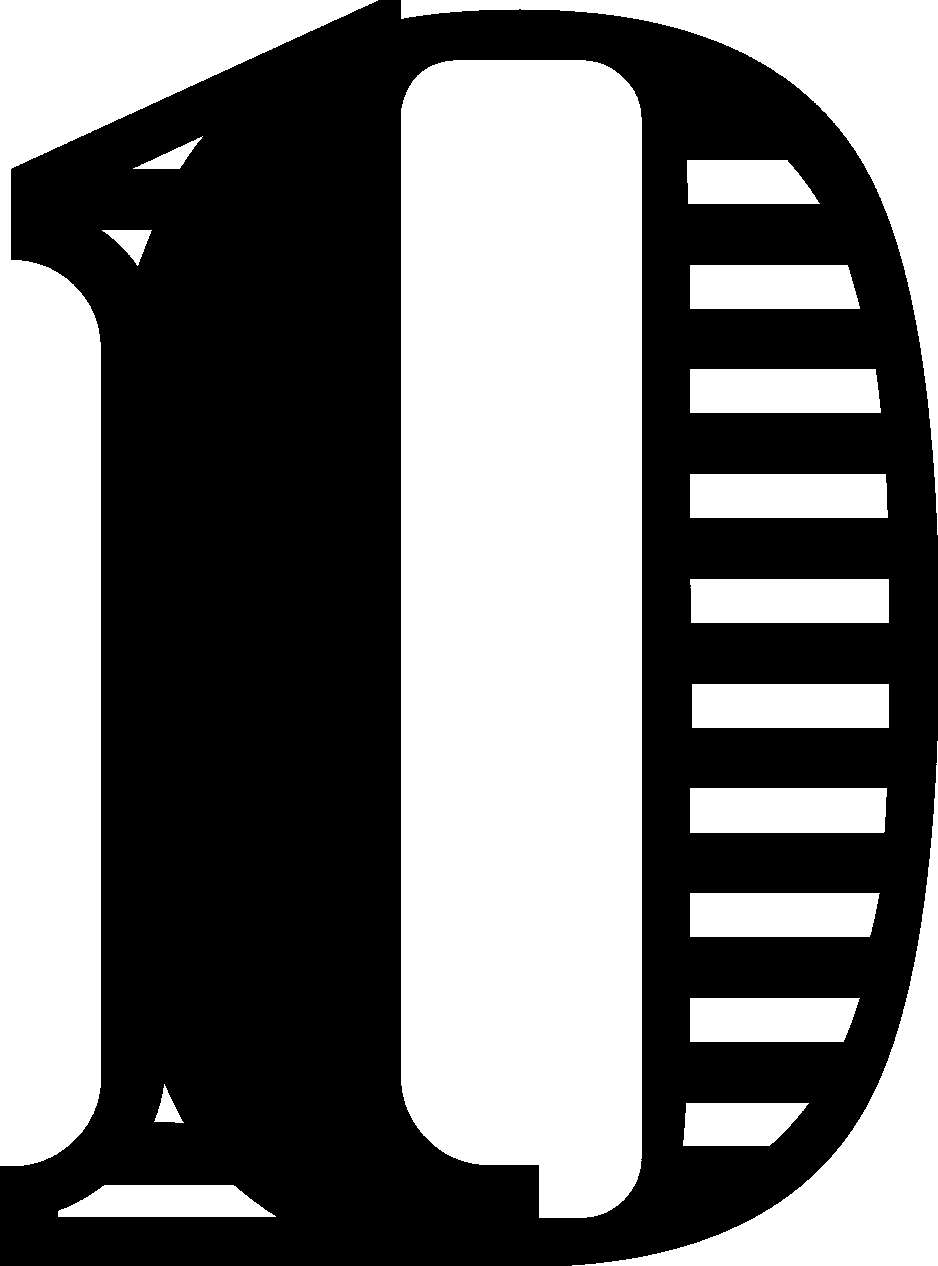
\includegraphics[width=\paperwidth]{./bilder/sektions_bilder/D.png}}
}

\begin{parse lines}[\noindent]{#1\\}

"Rosa på bal", vackert namn, eller hur?
Början i moll och finalen i dur
När blir den färdig, herr Andersson, säg,
visan ni diktar till mig?

Visan om er, fröken Rosa,
får ni ikväll till ert bord
Medan vi talar på prosa
diktar jag rimmande ord.

Tyst! Ingen såg att jag kysste Er kind
Känn hur det doftar från parken av lind
Blommande lindar kring månbelyst stig
Rosa, jag älskar dig!

\end{parse lines}


\subsection*{Störst och bäst} 
\index[alfa]{Störst och bäst}
\index[anfa]{Vem är störst och bäst i Skåne?}
\songinfo{Mel: Who's that lying on the runway?}

\begin{parse lines}[\noindent]{#1\\}
  Vem e störst och bäst i Skåne?
  Vem e kung på LTH? "ja LTH"
  Ja de e data infocom
  som hela festen drar igång
  tacka gud för data infocom!

\end{parse lines}

\vissteduattlong{Visste du att D-sektionen skapade Sveriges första studentwebb \\
och hade en hierarkiskt ordnad länksamling långt innan stora\\
sidor som Yahoo?}

\newpage
\resetBackground

\backgroundsetup{
  scale=0.50,
  opacity=0.15,
  angle=0,
  color=black,
  vshift=-180,
  hshift=110,
%   vshift=-230,
%   hshift=160,
  contents={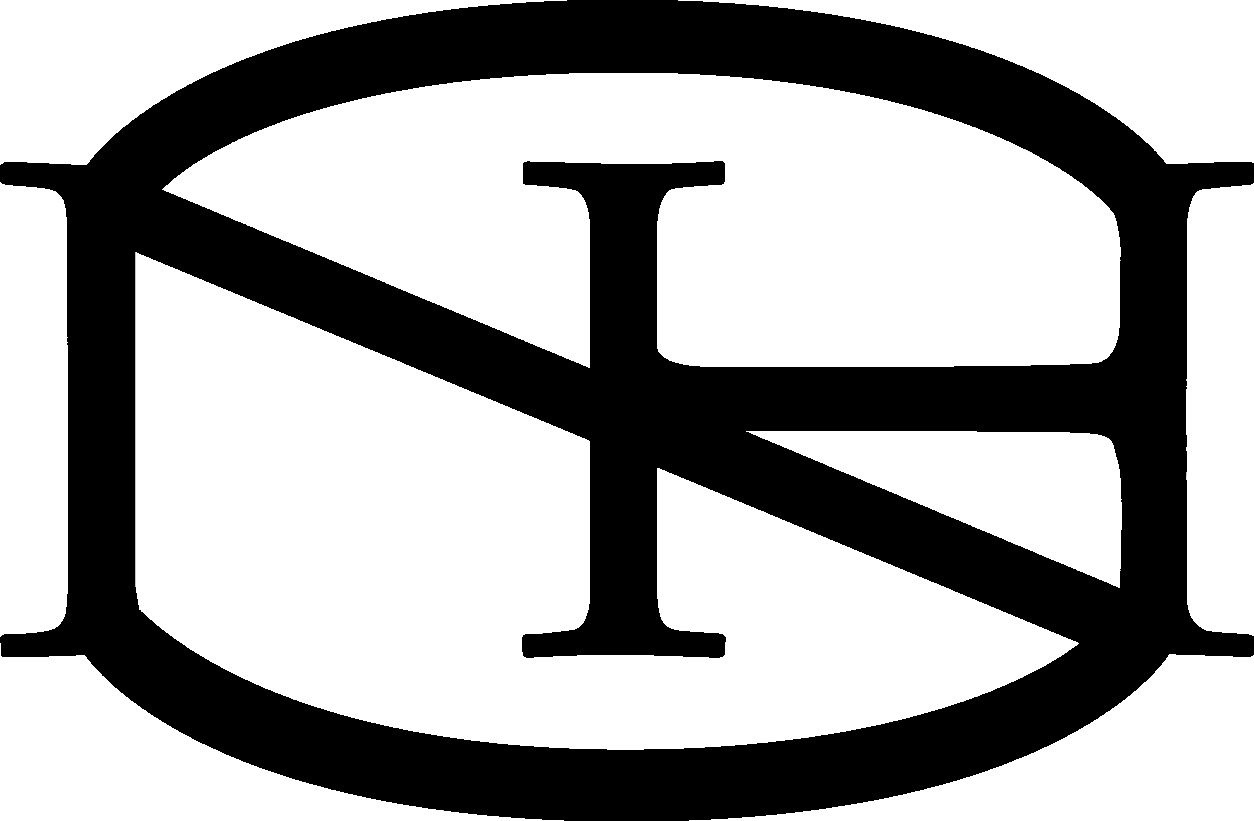
\includegraphics[width=\paperwidth]{./bilder/sektions_bilder/ING.png}}
}

\subsection*{Vi är ING-sektionen} 
\index[alfa]{Vi är ING-sektionen}
\index[anfa]{Vi är ING-sektionen}
\songinfo{Mel: We will rock you}

\begin{parse lines}[\noindent]{#1\\}
    Lundarna ni har det tråkigt utan oss,
men nu när vi är här kan ni släppa loss.
Vi känner ingen sorg,
Vi är från Helsingborg
vi super, festar, sjunger och spyr på era torg.

||: Vi är ING-sektionen :||

Byggteknik och data, de är så jävla vi.
Vi är inte dryga, men det är ju ni.
Vi kommer ner till Lund
Och roar er en stund,
Sen drar vi tillbaks till våran stad vid Öresund.

||: Vi är ING-sektionen :||

\end{parse lines}


\subsection*{ING från sundets pärla} 
\index[alfa]{ING från sundets pärla}
\index[anfa]{För vi är ING från sundets pärla}
\songinfo{Mel: Robin Hood Rooster song}

\begin{parse lines}[\noindent]{#1\\}
    För vi är ING från sundets pärla
    Och det är fest idag igen
    Och vi ska supa hela natten lång,
    och sjunga denna sång
    Shalalala…
\end{parse lines}

\vissteduatt{Visste du att FlyING 2014 hade sitt eftersläpp på Retro i Helsingør?}

\newpage
\resetBackground

\backgroundsetup{
  scale=0.50,
  opacity=0.15,
  angle=0,
  color=black,
  vshift=-180,
  hshift=110,
%   vshift=-230,
%   hshift=160,
  contents={
\includegraphics[width=\paperwidth]{./bilder/sektions_bilder/W.png}}
}

\subsection*{Turkosa samban} 
\index[alfa]{Turkosa samban}
\index[anfa]{Turkosa samban}
\songinfo{Mel: Samba de Janeiro}

\begin{parse lines}[\noindent]{#1\\}
    ||: Turkos Turkos här gör vi entré
    Vi bränner sprit uti KC:G
    Turkos Turkos så gör dubbel W
    Mitt glas är två för att jag är sne! :||
    ||: Simma sí, ah simma, ah simma simma simma :|| x4

\end{parse lines}


\subsection*{Hej här kommer W-sektionen} 
\index[alfa]{Hej här kommer W-sektionen}
\index[anfa]{Hej här kommer W-sektionen}
\songinfo{Mel: Segertåget}

\begin{parse lines}[\noindent]{#1\\}
    Hej här kommer W-sektionen
    sitter allra högst på tronen
    Pantar burkar, räddar världen
    och har jävligt kul på färden
    Äh vi kör igen!

\end{parse lines}

\vissteduatt{Visste du att TLTH har gett bort en livs levande hammarhaj som 
\\heter Daisy till W-sektionen som present?}


\newpage
\resetBackground

\backgroundsetup{
  scale=0.50,
  opacity=0.15,
  angle=0,
  color=black,
  vshift=-180,
  hshift=110,
%   vshift=-230,
%   hshift=160,
  contents={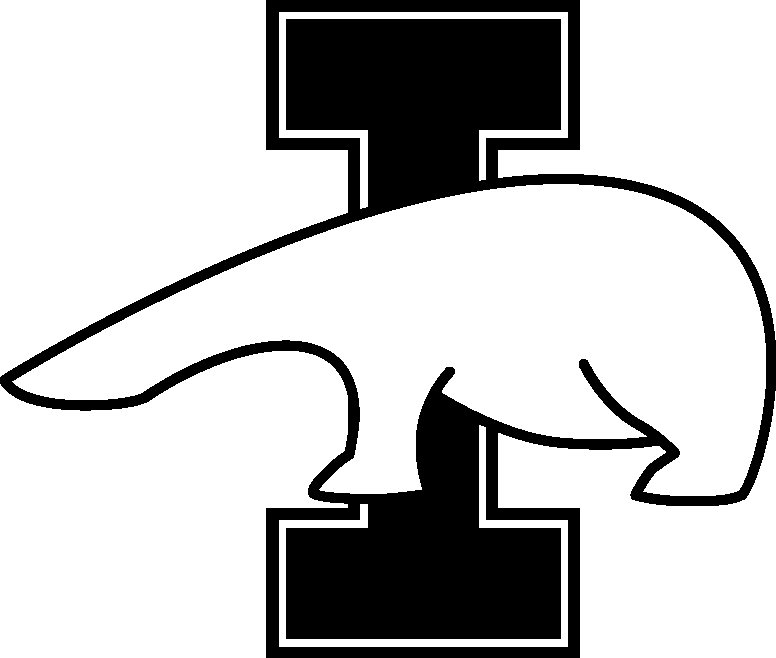
\includegraphics[width=\paperwidth]{./bilder/sektions_bilder/I.png}}
}


\subsection*{Bortom vägar och vatten} 
\index[alfa]{Bortom vägar och vatten}
\index[anfa]{Bortom vägar och vatten}
\songinfo{Mel: Pomp and Circumstance}

\begin{parse lines}[\noindent]{#1\\}
    Bortom vägar och vatten, 
    långt långt över Maskin,
    innan Brand hunnit släckas, 
    blickar vi ner på Kemi
    Bam bam bam!
    Stolta står vi och väntar,
    tills Elektro gjort sin sorti,
    för vi är bästa sektionen, 
    och vi älskar vårat I!
\end{parse lines}

\subsection*{Heja I-sek} 
\index[alfa]{Heja I-sek}
\index[anfa]{Heeey, Heja I-sek}
\songinfo{Mel: Hey baby}

\begin{parse lines}[\noindent]{#1\\}
    Heeey, Heja I-sek,
    Ooh, aah!
    Alla vill ha våran röda färg,
    I årgångsbordeaux!
\end{parse lines}


\subsection*{I-overall på} 
\index[alfa]{I-overall på}
\index[anfa]{I-overall på}
\songinfo{Mel: Millenium två}

\begin{parse lines}[\noindent]{#1\\}
    Åh, I overall på,
    Elitnivå,
    Top of the line på LTH
    Vi spårar som få,
    När I-Tåget köttar på!
\end{parse lines}

\vissteduatt{Visste du att I-sektionen är den enda sektionen på LTH med bara \\
ett program?}

\newpage
\noBackground

%\includepdf[angle=-90, pages=-]{./bilder/sektions_bilder/ny karta.pdf}
här ska det vara en bild på loftet
\newpage


